% (c) 2020 Stefan Antonowicz
% Based off of tex found at https://github.com/ludus-leonis/nipajin
% This file is released under Creative Commons Attribution-NonCommercial-ShareAlike 4.0 International License.
% Please do not apply other licenses one-way.

\renewcommand{\yggArbiter}{%
    \mychapter{Arbiter's Resources}{arbiter}
    \begin{center}
    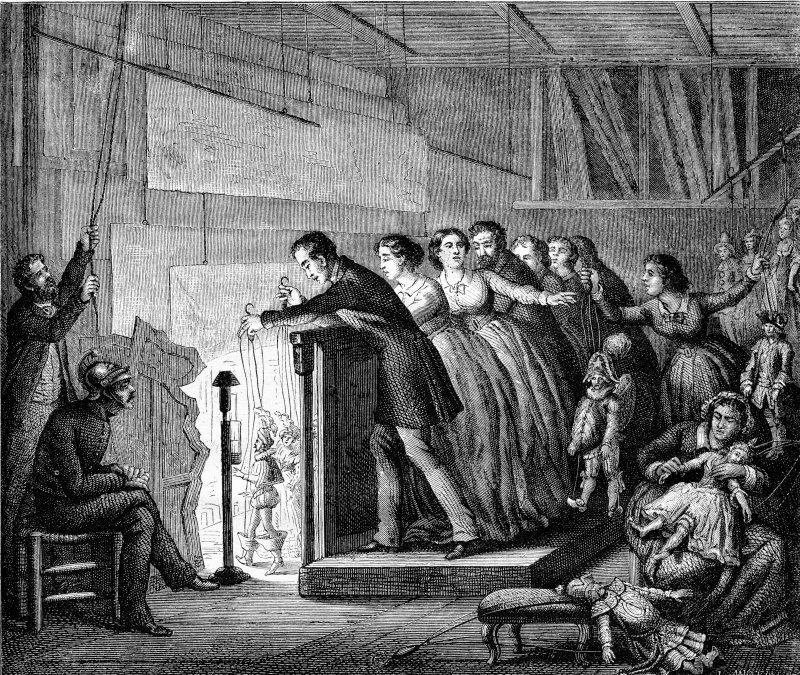
\includegraphics[width=\linewidth,keepaspectratio=true]{arbiter/ArbiterHeader}
    \end{center}
    \newpage
}


\renewcommand{\yggArbiterText}{%

\ed {
    This book started out as a bunch of house rules that I had cobbled together over the years, some of which had their origins in old Greyhawk campaigns I used to run. During what I'll call the "Google+" period of OSR, these house rules exploded into what you're holding in your hands. 

    This section is for the Game Masters, heart to heart. Everything that follows is completely optional, but I'm hoping these ideas show how you can leverage the ruleset to "attack the character sheet" of your players and give them a challenge. I've included a few handy checklists as well.  

}

\mysection{Adventuring}{arbiter-adventuring}

\mysubsection{The Movement Die}{arbiter-movement-die}

\mylink{Heavy Armor}{gear-armor} has a lot going for it, but there are some serious drawbacks too.  You should always know which Adventurer has the lowest Movement Die - they're going to be responsible for a lot of rolling.

\mybullet {

    \item \mybold{Sneaking:} Say the Adventurers are trying to sneak past the sentries of Cathedral of St. Aloysius of the Scourge, or slip out the door of the Bleeding Ram when the local authorities show up, or back up (quietly!) through the cave without waking the sleeping owlbears they just stumbled on.  Have the player with the lowest Movement Die roll - on a Failure, they are discovered.

    \item \mybold{Moving Quickly:} The players want to cross a room filled with something dangerous (swarms of shrieking crabs, mushrooms that release soporific spores when disturbed, a fire the Pooka started for reasons that aren't entirely clear).  Give the room a difficulty number to cross it (say 20) and tell them to start rolling their Movement Die - this represents how far they can travel in a Moment.  The results are cumulative; if you are unarmored and rolling a d20 and your first roll is a 12, you only need an 8 or better next time you roll to cross the room.  Obviously you can see that a lucky, unarmored Adventurer could conceivably cross the room in one Moment (by rolling a 20), while even the luckiest sad sack in plate mail is going to take at least 5 Moments to do the same.  Each Moment, have whatever the bad thing is in the room attack, deal damage, etc.

    \item \mybold{Contesting:} If two (or more!) Adventurers try to grab for the same thing at the same time (rushing to be the first to grab the evil relic, or catch the diamond skittering across the dance floor, or grab the falling vial of poison) have them \RB:\MD\@.  For more excitement, handle it the same way you handle the dangerous room above - set a number to get the item, and let them have at it.

    \item \mybold{Getting Chased:} Both the pursuer and the pursued need to \RB:\MD\@. The Adventurer with the lowest \MD rolls for the whole group, unless they get left behind (at which point it'd be the next lowest \MD, etc). The loser moves their \MD \DCDOWN, and the winner moves their \MD \DCUP (track this separately, this is just for the purposes of the chase).  The chase ends when someone loses on a d4 or wins on a d20.  During a chase, any Shoot or Throw attacks suffer a penalty equal to the opponent's \MAX \MD (-4 for a d4, -8 for a d8, etc). If the \myital{pursued} rolls a Failure on their \MD, the pursued can try to do something to "shake 'em" (jump into a pile of hay, slip into a crowd, spill an apple cart) - and if they win the next check, they escape. If the \myital{pursued} rolls a Failure on their \MD, they pursuer can do something to "stop 'em!" (yell at Old Man Bob to trip them, alert a good Samaritan or the authorities, etc.) - and if they win the next check, the chase is over.

}


\mysubsection{Burden}{arbiter-using-burden}

Don't ignore \mylink{Burden}{gear-burden}; use it to simulate heavy or unwieldy things including excess weight (the Morbid Obesity curse or what-have-you), or things that need to be carried by more than one person (my players liked to steal carpets for whatever reason. I used to say these rugs were 2-handed and had a Burden of 15, meaning they usually had to be carried by two people).  

\mysubsection{Hands and Tongues}{arbiter-hands-tongues}

It's ... weird how often this comes up:

\mytable {l c c X}{
    \thead{} & \thead{Hands Required} & \thead{Tongue Required} & \thead{Other} \\
} {
    Charms & 0 & No & You must be conscious \\
    Leechcraft & 2 & No & \\
    Liturgies & 2 & Yes & \\
    Remembrance & 0 & Yes & \\
    Sacraments & 1 & Yes & \\
    Whispers & 0 & Yes & \\
    Witchcraft & 1 & No & \\    
    Wizardry & 2 & Yes & You must be able to read (unless the Secret is inside of your skull). You can't be wearing/carrying iron. \\
}

\mysubsection{Iron}{arbiter-iron}

Iron is a "thing" in the Totality of Ygg. Spriggan are allergic to it and can't even touch it; Philosophers of a sorcerous persuasion can't practice the Secrets if they're in proximity to too much iron (a pocketful of iron pieces or an iron dagger is OK, but being wrapped in iron chains or carrying an iron longsword would be a problem).  This can make things difficult for these types of Adventurers, since tools, weapons, and (of course) iron pieces are made out of the element. If you have Spriggan or wizards in the Band, keep this info in the back of your mind!


\mysubsection{Luck Contests}{arbiter-luck-contests}

Sometimes you may need to figure out what random bad thing is going to happen to someone ("the ogre turns his attention towards one of you"; "one of you gets hit with 2 effects, not just one", etc. )

Tell your players to try \mybold{any} \mylink{Personality}{adventurer-personality} facet they choose, but instead of rolling the \UD, the player(s) can opt to "take a one" (meaning their roll is an automatic 1).  The player with the lowest roll is the victim. If there's a tie for last (including if multiple people decide to "take a one"), pick randomly or do whatever makes sense.

\newpage

\mysubsection{Persuasion}{arbiter-persuasion}

On occasion, an Adventurer may need to "persuade" a prisoner to tell them what they want to know, or do something they don't want to do. Obviously, the players need to be able to speak the language of the prisoner.  If they do, give the prisoner three aspects: 

\callout {
\mybullet {
    \item \mybold{Endurance} equal to the victim's \HD;
    \item \mybold{Resistance} equal to the victim's Morale; and
    \item \mybold{Will} represented by a number between 1 and 10.
}}

A cowardly goblin might have a Will of 1 - a demon might have a Will of 10.

If the prisoner's Resistance ever hits 20, there is nothing the players can do to make the creature give up the correct information (either they "buckle" and they didn't know anything to begin with, or they "feel pain as pleasure" or whatever TV trope you like). If the prisoner's Resistance hits 0, they'll give any information the players are after, or accept whatever belief the players want.

The base roll is an \RBTRY{\PRE}{Will}.  If the Adventurer wins, subtract the difference between their \PRE roll and Will from Resistance. If they lose, add it instead.

The Adventurer's have a few things they can do to better their chances:

\mybullet {
    \item \mybold{Torture:} the Adventurer adds +1 to their roll for each point of damage they do to Endurance (up to +4). Damage to Endurance isn't a die roll - the Adventurer simply states how much damage they wish to deal (between 1 and 4 points). If they lose the subsequent try, the Resistance gained by the monster is doubled. Remember that a Monster who is brought to 0 Endurance dies. 

    \item \mybold{Intimidation:} the Adventurer gains a +1 to +4 bonus to their try by roleplaying the questioning with you; depending on how convincing you think they are, give them the appropriate bonus.  If they lose the subsequent try, add the bonus to the Resistance gained by the monster. 

    \item \mybold{Seduction:} Includes bribery. The Adventurer gains a +1 to +4 bonus to their try by roleplaying the questioning with you; depending on how convincing you think they are, give them the appropriate bonus.  If they lose the subsequent try, add the bonus to the Resistance gained by the monster. 

    \item \mybold{Interrogation:} The Adventurer can use their Awareness instead of their Presence.
}

The Adventurer can only pick one technique (torture, intimidation, seduction, or interrogation). The players can work as a team, but only one person at a time can roll (i.e. they can play "Good Cop / Bad Cop" with a combination of Seduction and Intimidation, but only one person rolls the die using their Presence). No more than two Adventurers can "work" someone at a time.

Finally, the Adventurer can tend to the victim to try to keep them alive. The Adventurer "heals" between 1 and 4 points of Endurance; each point of Endurance healed increases Resistance by +1.


\example {
    The Band of the Big Toe captures two goblins and their hobgoblin leader, and hold them for questioning. The goblins have an Endurance of 1 (1 \HD) and a Resistance of 4 (Cowardly). The hobgoblin has an Endurance of 2 (2 \HD) and a Resistance of 8 (Orderly). I figure the goblins have a Will of 1, but the hobgoblin is a little braver and has a Will of 4. I don't tell the players though, just mark it down.  

\myskip

    They begin working over the first goblin, deciding to (unnecessarily) torture it for more information. They decide to do 2 points of damage to the creature's Endurance to get a +2 to their roll.  Since the goblin only had an Endurance of 1, they immediately kill it instead.  Whoops. On to the next goblin!

\myskip

    After a little discussion, they decide to let the barbarian take a crack at it. He has a \PRE of d6 and tells me he wants to Intimidate the critter. I ask him how, and we roleplay a bit - not a bad performance, I give him a +2 on his roll, and he rolls a 5+2 for 7 total, vs the goblin's Will of 1. The barbarian drops the creature's Resistance by 6 (7 - 1 Will); since it only had a Resistance of 3 it begins babbling everything it knows - which turns out isn't much.  They turn their attention to the Hobgoblin.

\myskip

    They try the same tack but the Hobgoblin has heard the spiel before, so I only give the barbarian a +1.  This time around he rolls a 1 (+1, 2 total) vs. the Hobgoblin's Will of 4. The difference is 2, so that's added to the Hobgoblins Resistance. In addition, a failed Intimidation roll adds to the Resistance, so that's another point. The Hob's Resistance is now 11 (8+2+1). He laughs and spits in the warrior's face. They try again, opting for a quick "torch to the groin", but only for 1 point of damage to the creature's Endurance (they're not entirely sure how much the thing can take). +1 to the roll, and the barbarian manages a 4 this time (for 5 total). The Hob's Resistance drops by 1 (to 10).  "I ain't tellin' you nuttin!! I can do this all day!"

\myskip

    While the party discusses whether or not they should continue, the sorcerer - moved by pity - sneaks over gives the Hob some water, and binds its wounds. The player tells me they want to "heal" 1 point of Endurance. They succeed, and I move the Hob's Resistance back up to 11 as well. 
}


\mysubsection{Mummy's Curse}{arbiter-mummys-curse}

This is a specific clarification but it came up enough to warrant a note. If a Knave has the \mylink{Virtue: Mummy's Curse}{knave-virtue-mummys-curse}, what are they allowed to do?

As long as the Knave intends to sell the item \mybold{and} isn't benefiting from the item directly, they can do what they wish with the item - including wearing it, sewing it into clothing, etc.  The Knave can't give a cursed item to someone - they \mybold{must sell it}.

That said, a cursed item can still be stolen from a Knave.  This can be through goading ("Heavens!  I hope these ruffians don't notice my mother's pearls!  They're a family heirloom!  Very old and valuable, you see...") or coercion, but the cursed item can't just be dropped or left out in the open for someone to "steal" (at your discretion).

\newpage

\mysection{Dungeon Crawling}{arbiter-dungeon-crawling}

\mysubsection{Light and Darkness}{arbiter-light-darkness}

\ed{This is shamelessly adapted from Patrick Stuart's \href{http://www.lotfp.com/store/index.php?route=product/product\&product_id=262}{Veins of the Earth}
}

In the dark, light is Init.  If someone isn't carrying a light, they have to be "with" someone who does.  If Magnuss is holding a torch, you can say "I'm with Magnuss", and be within the radius of light thrown by his torch.  You'll need to remain Close or Nearby the person you're "with" to be within the range of their light.

If you're holding a lamp, you lose the use of that hand - but you are now the "caller" for you and the people who are "with" you.  \mybold{Only people holding lights are allowed to roll Init.} The caller dictates the order in which anyone "with" them is allowed to go.

\example{Magnuss is holding a torch, and Kredique and Icarium are with him.  They happen upon a group of kobolds in the darkness.  Magnuss rolls Init and rolls a 24 - the Adventurers in this group go before the kobolds.  After a quick discussion, Magnuss states that Kredique will go, followed by Icarium, followed by himself}  

Note that creatures that act first in a Moment (Pooka, Spriggan, etc.) do not roll Init - their reaction time is otherworldly, and react faster than a others are capable of.  If a creature that doesn't roll Init is holding a light, they go first, but everyone who is with them automatically loses Init.

Finally, Adventurers with \mylink{Darksight}{effect-darksight} are able to roll their Init provided they're not "with" someone holding a light.

If an Adventurer drops a torch or lantern to free their hand, roll the item's \UD\@.  On a Failure (1 or 2), the \UD is moved \DCDOWN, and the torch or lantern goes out (a hireling \mylink{Linkboy}{gear-hirelings-linkboys} only fails on a 1). Linkboys have a \DEX of d8 for purposes of trying Init.

\mysubsection{Wandering Monsters}{arbiter-monsters-wandering}

\ed{Wandering monster checks make use of \href{Blades in the Dark's}{https://bladesinthedark.com/progress-clocks} revolutionary idea of the "progress clock".  I'm going to assume you're familiar with it, but if not - click on that link. It's an amazing tool to add to your arsenal.}

I break wandering monster checks into two types: active and resting. \mybold{Active} means people are banging around the dungeon, "whispering" to each other, stepping on feet, coughing from torch smoke, snickering at stupid jokes, and generally behaving like a group of kindergartners trying to be quiet.  \mybold{Resting} means the Adventurers are trying to take a \mylink{Bivouac}{combat-resting-bivouac}. 

\mybold{Active Checks}

Create a 6-segment progress clock. Fill in segments as follows:

\mynumlist {
    \item Set a timer for 20 "real world" minutes (if you want a more deadly dungeon, set it for 15 - if you want something a little easier, set it for 30).  Whenever the timer goes off, add a segment.  The timer is always running!  It only pauses (and resets) when the Adventurers take a Bivouac. Whenever the timer goes off, roll for light sources (see below).

    \item If the Adventurers "Quickly" search a room, add 1 segment; if they "Carefully" search a room, add 2 segments; if they "Thoroughly" search, add 3. "Quickly" searching reveals surface level things, "Carefully" searching reveals hidden things with a die roll (like a 1-in-2 for secret doors), and "Thoroughly" searching reveals all secret doors and treasure in a room.  Add one or two extra segments if the room is especially large or cluttered.

    \item If the Adventurers are making a lot of noise (more than normal, like trying to hammer down a door or take down a statue or something), add a segment.  Combat is noisy - getting into a fight adds a segment (which means, of course, that entering Combat might trigger a Wandering Monster check!) Prolonged or "extreme" combat (like if the Adventurers decide to explode something or set things on fire) bump this another 1-2 segments.
}

When the progress clock hits 6 segments, the Adventurers roll for a wandering monster.  The Adventurer with the lowest Movement Die is responsible for rolling; in the case of a tie, the players can choose.  The Adventurer rolls their Movement Die - on a Failure (a 1 or a 2), a Monster wanders by (the rationale is that the guy in plate mail is making a lot more noise than a group of unarmored thieves and wizards, but if you find this too harsh use a d6 or a d8 instead). Reset the progress clock and continue play (but note that this doesn't pause the 20-minute "real world" timer!) 

Additionally, every time you reset the progress clock:

\mybullet {
    \item Adventurer's roll their \UD for torches. If they fail, their \UD moves \DCDOWN, and they have light another (if you're a nice Arbiter, let them roll for wandering monsters before they roll their \UD). Put a token on or near the progress clock.

    \item If there's a token on or near the progress clock (that you haven't just placed there), have them roll their \UD for lanterns (oil).  If they fail, their \UD moves \DCDOWN. Remove the token.
}

Keep the clocks and timers out in the open - like the Sword of Damocles, the palpable sense of danger will hang over their heads and hopefully keep them moving and making rushed decisions, and that's where the magic happens ...

\mybold{Resting Checks}

I figure a "long rest" or bivouac is about 8 hours, so I'd make two monster checks (provided the party didn't have a \mylink{Pooka}{species-pooka} or  \mylink{Hearthfire}{arcana-mystery-hearthfire} or something like that).  If they Adventurers didn't post a guard and a wandering monster showed up, it automatically gets the Drop on them.

Base chance of a monster is 1-in-6 (17\%). Roll a one, flip a coin - heads the monster shows up in the first half of the watch, tails it shows up in the second half. In more heavily trafficked areas, I might use a d4; if I wanted to give the Adventurer's a break (or they took precautions of some sort), I'd bump it to a d8.  

Remember the Adventurers heal Grit right away when taking a Bivouac, but they \mybold{don't} get any of the other bonuses for resting until the Bivouac is complete (meaning that if a monster finds them while they're resting, they won't necessarily be completely healed up).

Remember to pause the "Active" timer, and reset it when the Bivouac is over.



\mysection{Combat}{arbiter-combat}

\mysubsection{Ebb and Flow of Combat}{arbiter-combat-ebb-flow}

I just wanted to link to the Angry GM's \href{https://theangrygm.com/manage-combat-like-a-dolphin/}{Manage Combat Like a Motherf\$\&\%ing Dolphin}, since the ToY combat system is based around this concept. The combat system is designed for you to be as narrative as possible, by taking a lot of the dice rolling for monsters out of your hands. There's no Init for monsters, they don't roll attacks (spells notwithstanding); really the only things you'll need to roll are damage and saves.  This gives you a lot of opportunity to narrate combat, strategize your beasties, and interact with the environment. 


\mysubsection{Alternate Grit}{arbiter-alternate-grit}

Remember that Grit represents the Adventurer's will to fight. If you want, you can make Grit a little more dynamic in Combat to encourage players to do cool shit. Give them a few points of Grit (even above \MAX):

\mybullet {
    \item every time they Crit, or;
    \item every time they kill a monster, or;
    \item every time they do something rad;
    \item etc.
}

the inverse is true too, you can have certain effects and terrible, horrible things rob them of Grit. Just a reminder that any Grit above \MAX disappears when they take a Bivouac.


\mysubsection{Dueling}{arbiter-rules-dueling}

\ed{I know I adapted this from somewhere, but I don't remember where. If you're the author, please let me know!}

\begin{wrapfigure}[9]{l}{0.4\textwidth}
    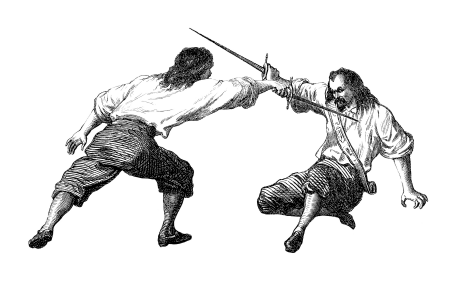
\includegraphics[width=0.4\textwidth]{arbiter/CombatDuel}
\end{wrapfigure}

This is if you want to add a little extra something to a duel between an Adventurer and a Monster (or two Adventurers!)

Take a set of 3 index cards for each combatant.  On each set, write the following (1 per card)




\mybullet {
    \item Feint
    \item Parry
    \item Push
}


and place them in front of each combatant. At the top of each Moment (before you roll Init), each combatant flips a card. Roll Init and apply the following bonuses:

\mybullet {
    \item FEINT beats PARRY.  The winner gets a +4 on their Attack try.
    \item PARRY beats PUSH.  The winner gets +4 on their Guard roll.
    \item PUSH beats FEINT. The winner gets +4 on their damage (if they hit).
}

If there's a tie, \myital{both sides} get the bonus (both Feint: +4 Fight; both Parry: +4 Guard; both Push +4 damage)

\mysubsection{Combat Keywords}{arbiter-combat-keywords}

A good Adventurer should use their environment to their advantage as much as possible. It can be useful to use "combat keywords" to describe a room or scenario when combat is first joined.  The Arbiter should attach two or three adjectives to each Combat, and improvise based on these keywords.

\example{The adventurers creep through a tunnel into the lair of a salamander.  The Arbiter describes the area using the combat keywords "crowded", "dazzling", and "ovenlike". Using Whispers of the Bride might have a higher Target because it's "dazzling"; you might only lose a Blood die on a 1 if you use Fireball, but Icebolt will deal -1 damage per die because of the "ovenlike" conditions, etc.}

\mytable{X X X X}{
    \thead{Scene} & \thead{Lighting} & \thead{Conditions} & \thead{Terrain} \\
}{
   austere & bright & acidic & bouldered \\
baronial & burning & acrid & cloudlike \\
barren & clear & arctic & earthen \\
burnt-out & cloudy & arid & flat \\
carpeted & dark & bitter & grassy \\
cavernous & dazzling & bloody & greasy \\
cluttered & foggy & boiling & hard \\
comfortable & ghostly & choking & icy \\
crowded & glistening & cold & irregular \\
derelict & glittering & dank & jagged \\
dilapidated & light & dirty & jumbled \\
dusty & luminous & dry & loose-footing \\
furnished & misty & fiery & marshy \\
haphazard & murky & frigid & muddy \\
}

\newpage

\mytable{X X X X}{
    \thead{Scene} & \thead{Lighting} & \thead{Conditions} & \thead{Terrain} \\
}{

labyrinthine & radiant & gaseous & pebbly \\
lofty & shadowy & gusty & porous \\
messy & shady & hot & rocky \\
neat & shimmering & humid & sandy \\
palatial & smoky & icy & slick \\
ruined & sparkling & moist & slimy \\
snug & sunlit & moldy & slippery \\
spacious & unshadowed & muggy & smooth \\
spiderwebbed & vaporous & ovenlike & spongy \\
sprawling &  & rainy & stony \\
stuffy &  & rusty & swampy \\
unfurnished &  & salty & tree-lined \\
well-appointed &  & scorching & uneven \\
 &  & sizzling & unstable \\
 &  & sooty & yielding \\
 &  & steaming &  \\
 &  & steamy &  \\
 &  & stinking &  \\
 &  & swarming &  \\
 &  & sweltering &  \\
 &  & tropic &  \\
 &  & wet &  \\
 &  & windy &  \\
 &  & wintry &  \\
} 



\myimage{arbiter/MonsterDinosaurFight}

\newpage

\mysection{Monster Creation}{arbiter-monster-creation}

\ed {
    A level 1 monster does an average of 3.5 points of damage with a maximum of 6 - meaning that on average the weakest combat class (Philosopher) will be able to take a hit without taking Flesh damage, and in the worst case be able to take max damage without immediately dying.

    Monster average damage goes up an average of 1 to 1.5 points per level, though the deviation increases, making damage from fighting higher \HD monsters more "swingy".  Max damage increases by 2 points per level (the exception being 9 \HD monsters, where max damage increases by 5).
 
}


Monsters should map 1-to-1 to Adventurer's in terms of challenge i.e. a 1 \HD monster should be a challenge for a Level 1 Adventurer. For reference:

\mytable{X c c c c c X}{
    \thead{} & \thead{\HD} & \thead{Damage} & \thead{Weak.} & \thead{Save} & \thead{Spells\Dagger} & \thead{} \\ 
}{
    & 0\Asterisk & d4 & d24 & 12 & 0 & \\
    & 1 & d6 & d24 & 11 & d4 & \\
    & 2 & d8 & d20 & 10 & 2d4 & \\
    & 3 & d10 & d20 & 9 & 3d4 & \\
    & 4 & 2d6 & d16 & 8 & 3d4 & \\
    & 5 & d6+d8 & d16 & 7 & 4d4 & \\
    & 6 & 2d8 & d12 & 6 & 4d4 & \\
    & 7 & d20 & d10 & 5 & 5d4 & \\
    & 8 & d10+d12 & d8 & 4 & 5d4 & \\
    & 9 & d24+d3 & d4 & 3 & 6d4 & \\
}

Some guidelines I use when I'm creating or converting beasties:

\callout {
\mynumlist {
    \item First step is to place the monster in an \mylink{Order}{monster-orders}, which will give them a few \mylink{Traits}{monster-traits} to work with. 
    \item After that, I usually give the monster an additional Trait, Combat Action, or Soak(d4) for "free."  Additional abilities will either nerf their damage or Power.
    \item Damage is based on 1 monster fighting 1 Close Adventurer. If you want to increase the number of targets (2 Close, for instance) or the range (1 Nearby), reduce the damage \DCDOWN on the chart above.
    \item Keep in mind that in hand-to-hand combat, it's challenging for anyone to do more than 10 points of damage to a monster. On average, a level 1 Adventurer should be able to kill 1 \HD Weak monster in 1 hit; an Average monster in 2; and a Strong monster in 3 hits (assuming they're using something that does d6 damage).
    \item If the monster can cast spells, add an additional spell to their repertoire at 3, 6, and 9 \HD.
}}



\newpage

\mysection{0-Level Adventurers}{house-rules-level-0}

\ed{The idea of the "character funnel" comes from Dungeon Crawl Classics. Honestly, it's some of the most hilarious gaming you can do. You create 2-4 hapless 0-level "Adventurers" per player, and run them through an adventurer. Mayhem and death abounds!}

\mybold{Character Creation}


\mybullet {
    \item Mortals only, I'm afraid. The non-Mortal species are busy escaping slavery / gestating in a fetid swamp / running through the fields of Elfland / etc.
    \item Define your Identity, Personality, Skills, and Saves. Don't worry about Kismet.
    \item Roll a d3. If you roll a 3, roll a d4. If you roll a 4, roll a d6 etc. Move up the dice chain until you don't roll \MAX, or you reach a d20. This is your Destiny die. You can use it as if it were a \mylink{Lucky Die}{knave-lucky-die} (add its result to any non-Combat \RO or \RB attempt) but it moves \DCDOWN \mybold{every time} you use it (not just if you roll a 1 or a 2).
}

\mybold{Equipment}

You can have \myital{one} of the following:  

\mybullet {
    \item  a makeshift 1-H \DEX Brawl weapon (sharpened rib bone, half-pair of scissors, stick) that does d4 damage.
    \item  a makeshift 2-H \VIG Brawl weapon (pitchfork, woodsman's axe, big stick) that does d6 damage.
    \item  a set of Light "armor" (patchwork leather jacket stuffed with straw, thick layer of mud, wooden barrel on suspenders) that has \UDD{d4}.
    \item  a peasant's "holy item" (simple wooden cross, sprig of holly, chicken foot). The holy item contains a single (d4) Grace Die. You (and only you) can use this Grace die to perform any of the \mylink{Sacraments}{vulgate-sacraments}.
    \item  a \mylink{Fetish}{fetishes} inscribed with a random Secret. You are able to read this Secret from inside the skull, but no others. Use your Destiny die as if it were a Blood Die to perform the Secret (don't forget to roll the \UD of the Fetish every time you use it).
}

\mybold{Death and Dying}

Pretty simple - whenever you're struck by something that can kill you (Arbiter's discretion), roll an appropriate Save (Hexes for magic, Toxins for poisons, Doom for everything else). If you succeed, you live. If you fail, you die.

\newpage

\mybold{I Made It!}

In addition to any goodies they find along the way, the Adventurer should roll their Destiny die. One. Final. Time.

\callout {\footnotesize{
\mybold{1-5}: At least you made it, right?

\mybold{6-10}: Pocketed that bauble when no one was looking. Roll for jewelry on the \mylink{Random Treasure Chart}{appendix-a-jewelry}.

\mybold{11-15}: That weapon you found / started with / given to you by the Arbiter as a reward for completing the meat grinder?  It's magical (counts as a magic weapon). 

\mybold{16-19}: You came out ... changed. Start with +d6 Grit.

\mybold{20}: Blessed by the Small Gods. You have the Virtue \mylink{Sacred Flesh}{mystic-virtue-sacred-flesh} (+2 Flesh, \DEATH moves to Tough(d4)). You can only choose this Virtue once (meaning if you create a Mystic, you can't choose this Virtue a second time).
}}

After you've rolled your Destiny die, create an Adventurer as normal (but skip Identity, Personality, Skills, and Saves).

    


\newpage


  \mysection{Checklists}{arbiter-checklists}

  \mysubsection{Session Checklist}{session-checklist}

  \mybold{At the start of the Session:}


  \mychecklist {
    \item Have any addicts roll their \mylink{Narcotics}{gear-narcotics} \UD so they can get their "fix".  If they don't have the narcotic on-hand, they are \mylink{Sickened}{effect-sickened} for the rest of the Session (\mylink{Leechcraft: Pharmaceuticals}{leechcraft-pharmaceuticals} can alleviate the effects).
    \item Remind everyone that Arcana and effects that last "one Session" have now expired. Abandoned have gone back to where they came, certain Liturgies are over, etc.
    \item Write down any effects or modifiers the players might have from Wounds, Curses, etc.
    \item Ask for everyone's \MD\@. 
  }

  \mysubsection{Combat Checklist}{combat-checklist}

  \callout {
      \mybullet {
        \item If an Adventurer rolls \mybold{minimum} damage, \RSTRY{\FOC}. Failure is a \mylink{Fumble}{combat-crits-and-fumbles}.
        \item If an Adventurer rolls \mybold{maximum} damage, \RSTRY{\FOC}. Success means a \mylink{Crit}{combat-crits-and-fumbles}.
        \item If an Adventurer is \mylink{Dying}{combat-dying}, roll for a \mylink{Wound}{physical-wound} right away - it might affect their Breather.
      }
   }


\begin{multicols*}{2}

  \mybold{At the start of combat:}

  \mychecklist {
    \item  Place the Adventurer and Monster tokens in the appropriate range bubbles.
    \item  Make a call on whether or not the Adventurers or the Monsters have \mylink{the Drop}{combat-drop}.
    \item  Check to see if anyone has any additional effects that must be rolled just before the Init phase.
    \item  Have everyone roll Init.  Pookas automatically win Init. 
  }

  If you're using the optional \mylink{Light and Darkness}{arbiter-light-darkness} rules, only the people holding torches roll Init.

\cbreak

  \mybold{During Combat:}

  \mychecklist {
    \item  Players roll Init.  If there are Monsters of different speeds (Fast and Slow, for example), roll in descending order (roll Init vs. Fast, then roll Init vs Slow).  If you \RO Init, stop.
    \item  Check for "top of the Moment" effects before an Adventurer acts.
    \item  Adventurers who \RO Fast Monsters go first.  Then Fast Monsters. Adventurers who beat Average Monsters, then Average Monsters, etc. Adventurers who failed all their \RO attempts go last.
    \item  Resolve combat
    \item  Check for "bottom of the Moment" effects (including Duration effects)
  }


\end{multicols*}


  \mybold{After Combat:}

  \mychecklist {
    \item Have anyone who survived Dying roll their \INSANITY and \INJURY dice.
    \item Check to see if anyone has any \mylink{Wound}{physical-wound} and make note of them.
    \item Ask if they want to take a Breather.
  }



  \mysubsection{Resting Checklist}{resting-checklist}

  \mybold{Taking a Breather}

  \mychecklist {
    \item Everyone restores 4 Grit up to their \MAX (unless prevented by Injury).
    \item Ask if anyone is taking Narcotics (make sure to check for Overdose).
    \item Check for additional healing effects (Pooka, Cuckold's Courage, etc.)
    \item If there's a Pooka in the party, ask them if they want to restore the Band's Grit.
    \item Sellswords with \mylink{Second Skin}{sellsword-virtue-second-skin} can repair 1 \UD of Armor (up to \MAX).
  }

  \mybold{Taking a Bivouac}

  \mychecklist {
    \item Collect a \UD roll against Personal Provisions for each person resting.  Anyone who doesn't make the roll gets none of the following benefits.
    \item All Adventurers restore 1 Flesh. 
    \item All Adventurers set their Grit to \MAX (if a Wound doesn't prevent it). If their Grit is higher than \MAX, the effect ends.
    \item All Adventurers restore 1 \UD of \mylink{Armor}{gear-armor}, up to its \MAX.
    \item All Adventurers restore 1 \UD of \myital{one} aspect of \mylink{Personality}{adventurer-personality}, up to its \MAX.
    \item  Adventurers restore some \POOL or \UD depending on their Flavor:
  }

    \callout {
      \mybullet {
        \item Restore \DCUP of your \mylink{Prowess}{sellsword-prowess}.
        \item Restore \DCUP of your Lucky Die (\mylink{Knave}{knave-lucky-die} or \mylink{Pooka}{pooka-lucky-die}).
        \item Restore \DCUP of your \mylink{Juju}{cruces-mojo-juju}.
        \item Restore \DCUP of your \mylink{Ingenuity}{cruces-knowledge-ingenuity}.
        \item Restore 2 \mylink{Blood Dice}{cruces-blood-dice}.
        \item Restore your \mylink{Grace Die}{vulgate-sacraments-grace}.
        \item Restore 1 point of \mylink{Sovereignty}{remembrance}.
      }
    }

\newpage

  \mybold{Taking Downtime}

  \mychecklist {
    \item Shopping Step. Handle anything they want to sell, and charge them for the stay (Days, Weeks, or Months). If they want or need to heal any wounds, madness, etc. handle that now.
    \item Resting Step. Restore stats, Grit, and Flesh to full.
    \item Production Step. Allow players to spend Research Pips and Cunning Pips; Spriggan can create magic swords.
    \item Training Step. Allow the players to convert coin to Glory.
    \item Arbiter's Choice. Assign any additional Glory you think is appropriate.
    \item Check if anyone gained a level.
  }


  \mybold{Gaining a Level}

  \mychecklist {
    \item Have the player roll all their Kismet dice. Add their total to the Adventurer's Grit.
    \item Have the player pick 3 appropriate Virtues.
    \item Assign any additional \mylink{Arbiter's Awards}{advancement-arbiters-awards}.
  }

} %end
